\documentclass[10pt,a4paper]{report}
\usepackage[utf8]{inputenc}
\usepackage{amsmath}
\usepackage{amsfonts}
\usepackage{amssymb}
\usepackage{fancyhdr}
\usepackage{tikz}

\usetikzlibrary{positioning, arrows, backgrounds, fit}
\usepackage{titlesec, blindtext, color}
\newcommand{\hsp}{\hspace{20pt}}
\titleformat{\chapter}[hang]{\Huge\bfseries}{\thechapter\hsp}{0pt}{\Huge\bfseries}

\newcommand{\attr}{\vspace{1ex} \hrule \vspace{1ex}}

\begin{document}
\chapter{Augmented Chess:\\ Assignment 6}

\begin{center}
{\Large \textbf{Group Members}}

\begin{tabular}{l r}
Jacob Holm Mortensen            &       jmorte14@student.aau.dk\\
Martin Raunkjær Andersen        &       marand13@student.aau.dk\\
Thomas Gwynfryn McCollin        &       tmccol14@student.aau.dk
\end{tabular}
\end{center}

\section{Question 1}
\begin{quote}
Consider at least two options for the following elements of your Web application, then make a choice and justify it
\end{quote}
The question will be answered with respect to the following elements. At least two options for each of the elements are considered.

\subsection{Programming Language}
Due to our choice of framework we narrowed down the choice of language to \texttt{JavaScript} or \texttt{TypeScript}. These are the languages supported by our chosen framework.

The advantages of \texttt{JavaScript} is the lower level of the language with respect to \texttt{TypeScript}. There is no compilation necessary, therefore the code we write is the code running on the client side. This affords developers more control and concrete understanding of the running code.

On the other hand \texttt{TypeScipt} is a more abstract language, this eases development and reduces development complexity. Furthermore typed languages are easier to support using external tools such integrated development environments. This also renders the code more readable. \texttt{TypeScript} is compiled to \texttt{JavaScript} therefore it will run in all common web browsers.

We have chosen to write the application in \texttt{TypeScript}. The language enables a sufficient understanding of running code, while significantly reducing development complexity. Furthermore it is supported by the framework, which affords the language additional construct that further reduce development complexity.

\subsection{Web Server}
For the mini-project we will be utilising a web server owned by a group member. This server runs Linux and the web serving is handled by a Node back-end. Since we are interested in reducing cost and complexity this is the optimal option available. However we will discuss an alternative.

Instead of running a Node back-end we could use another Linux based web server such as nginx. This means that our back-end must be handle requests and manage queue and game representations on the fly.

It is much simpler to use the Node back-end since the language on the back-end the front-end will be the same. Either \texttt{JavaScript} on the server side or \texttt{TypeScript} compiled to \texttt{JavaScript} on the client side.

\subsection{Framework}
For the choice of framework we have compared frameworks that the group has previous experience with and WebRatio. The frameworks we have some experience with are Angular and ASP.NET, however we will focus on Angular and WebRatio.

WebRatio is a graphical representation tool for \texttt{WebML}. The software and model are new to all members of the group. Furthermore, using WebRatio has been problematic, both in the case of running and the case of operating WebRatio. We estimate that the additional operating complexities of WebRatio outweigh the gains, in relation to this mini-project. 

Whereas a member of the group is experienced with Angular and other members have experience with web technologies such as \texttt{JavaScript}, \texttt{HTML} and \texttt{JSON}. This means that Angular has a much smaller setup complexity. This reduced complexity will allow us to develop a less trivial application in the limited time span of this project.

Due to the additional complexity of using WebRatio we have opted to use a framework that group members are somewhat or very familiar with.

\section{Question 2}
\begin{quote}
Describe the conditions under which you would choose hosting, housing or having your own Web server for your Web application.
\end{quote}

Our application will be running some application code on the back-end, such as the game queue and game management. Therefore the choice is either a enterprise level hosting service or self hosting the application.

Advantages of enterprise level hosting services are that resources and availability are guaranteed. Furthermore these are not the responsibility of the developers. This frees up time to evolve or maintain the application further. The downside of enterprise level hosting services is that they are very expensive.

Self hosting affords us greater control over resources and availability, however it also makes us responsible for them. A greater understanding of back-end related technologies is also required. However, self hosting the application is much less expensive. The cost consists of hardware acquisition cost hereafter is much smaller.

We have a small web server available and therefore we will opt for the self hosting solution. This is mainly motivated by the cost of enterprise level self hosting services and since we already have access to a running web server we may skip some of the complex setup steps usually involved with self hosting.

\section{Question 3}
\begin{quote}
Consider the activities described in Section 7.4.1 of "Engineering Web Applications" for a Webmaster. Which of these activities are the most time consuming and require domain knowledge or human participation and which ones could be automatized using tools?
\end{quote}
Each activity is listed and the possibility of automation is discussed as well as the estimated time cost.

\subsection{Conflicting Style}
Tools such as a simple web crawler could be used to search the website for pages that may contain conflicting styles. This crawler would only be able to estimate style conflicts and should report back every time a potential style conflict is found. Additionally users could report pages not conforming to the style guide.

\subsection{Inappropriate Content}
New content can be checked for a number of keywords or file types that are associated with inappropriate content. Whenever something is flagged the webmaster or a moderator should accept or reject the content. Users may also report inappropriate content. Additionally uploaded files may be scanned using virus scanning tools to prevent spread of malicious code using the website.

\subsection{Broken Internal Links}
This task may be solved using a similar or the same crawler as the first activity. Whenever a internal link is followed that leads nowhere the webmaster should be alerted, optionally also the user. The link should then be fixed by the webmaster or user.

\subsection{Broken External Links}
This task is difficult to automate since the automaton needs to understand the expected content of the external site. Therefore some testing can be automated, such missing pages. However if the content of an external site changes, but the link still works the crawler will be of little use. Either the webmaster should periodically check these links or let users report them when they are broken.

\section{Question 4}
\begin{quote}
From the extensions to your Web application proposed in the assignment 5, which ones could be considered as "maintenance changes" and which ones as "evolution changes"? Why?
\end{quote}

Both of the extension suggested in assignment 5 are evolutions of the application. The first extension was an additional feature enabling users to see the best players on a public leader-board. This a completely new feature that is not supported in the current system. The second extension is also an evolution. It is new user created custom board to play chess on. There is a subset of maintenance related tasks involved in this extension, however bulk of the extension consists of new functionality.

\section{Question 5}
\begin{quote}
Start or continue the implementation of your Web application. Focus on the main use cases. Briefly report the status of the development.
\end{quote}
Implementation of all views has begun. The navigation structure between these views is mostly finished. Implementation of the main features is underway. The first deliverable is to fully support a local game of basic chess. This has been partially implemented. We estimate that we will finish this deliverable before the end of next week.

Basic chess is defined as chess with correct move and attack rules. Additional rules such as en passant, castling and win conditions will be included in the next deliverable.

\section{Question 6}
\begin{quote}
Enhance your application design considering one of the extensions proposed in the assignment 5.
\end{quote}

To support either of the proposed extensions we would need to add an additional component supporting the new functionality. In the case of the leader-board two different approaches are viable. The leader-board could be a view on it's own, in which case it should be included in the hypertext structure and the a representation of the leader-board containing the best players should be added to the data model. Alternatively the new view could be omitted and the leader-board could be displayed on the main screen instead, in this case the data model would still need to be updated. In the following diagram the additions to the data model and hypertext structure can be seen. The green boxes are data objects and the blue boxes are pages. These diagrams should be considered additions to the previous diagrams.

\makebox[\textwidth][c]{
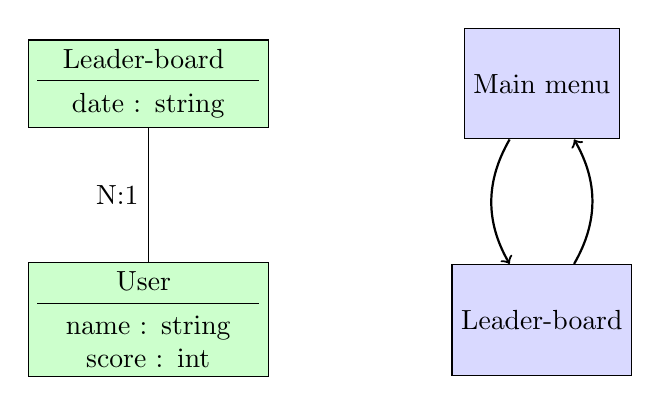
\begin{tikzpicture}
\tikzstyle{object}=[draw, rectangle, fill=green!20, text centered, minimum height = 3em, minimum width = 5em, text width = 8em]
\tikzstyle{page}=[draw, rectangle, fill=blue!15, text centered, minimum height = 4em, minimum width = 4em]
\tikzstyle{line}=[draw, ->, >=open triangle 90, thick]
\tikzstyle{link}=[draw, -latex, thick]

\node[object](leader-obj) at (0, 0) {Leader-board \attr date : string};
\node[object](user) at (0, -3) {User \attr name : string score : int};
\path[draw] (user) edge node[left]{N:1} (leader-obj);



\node[page](main) at (5, 0){Main menu};
\node[page](leader) at (5, -3) {Leader-board};
\path[link](main) edge[bend right=30, ->] (leader);
\path[link](leader) edge[bend right=30, ->](main);

\end{tikzpicture}}

In the case of the custom board extension, a larger modification is necessary. The game component needs to modified such that the rules can account for boards that are not square and then a new component needs to be added. This new component should be accompanied by a new view where users can create boards. The view should be added to the hypertext structure and the data model should account for a new object, boards. This object should consist of a set of cells, which have positions.

\makebox[\textwidth][c]{
\begin{tikzpicture}
\tikzstyle{object}=[draw, rectangle, fill=green!20, text centered, minimum height = 3em, minimum width = 5em, text width = 8em]
\tikzstyle{page}=[draw, rectangle, fill=blue!15, text centered, minimum height = 4em, minimum width = 4em]
\tikzstyle{line}=[draw, ->, >=open triangle 90, thick]
\tikzstyle{link}=[draw, -latex, thick]

\node[object](board) at (0, 0) {Board \attr author:string type:string cells:int};
\node[object](cell) at (0, -3) {Cell \attr colour:string position:string};
\path[line] (cell) ->node[left]{N:1} (board);


\node[page](main) at (5, 0){Main menu};
\node[page](creator) at (5, -3) {Board Creater};
\path[link](main) edge[bend right=30, ->] (leader);
\path[link](creator) edge[bend right=30, ->](main);

\end{tikzpicture}}

\section{Question 7}
\begin{quote}
Using the most elaborated page of the prototype produced for the assignment 3, specify its features using tags (step 3 in the MockupDD iteration). Compare this annotated mockup with the models in your Web application design. Identify the features covered by the annotated mockup. From the uncovered ones, which ones cannot be covered? Why?
\end{quote}
The prototype from assignment 3 consisted primarily of \texttt{navigation/interaction} tags. However the login, manage armies and game components where also tagged with \texttt{content} tags, since information is edited in these components. The components where fairly simple and consisted of links and some buttons. However the game component is much more complex. A number of pieces are present on the board that the user may interact with. This component is a composite widget made up of draggable elements.

The links, navigation and the management of armies is coverable by annotations, however the game component is more complex. A composite widget is best fit, however it does not fully reflect the behaviour of the game component.
\end{document}